\documentclass[conference]{IEEEtran}
% Tectonic compiles with XeTeX, which has no definition for IEEEtran's Times, Helvetica and Courier
% (ptm, phv, pcr). Without the lines below, LaTeX falls back to Latin Modern regular for every text font,
% losing bold, italics, small caps and monospace. The TeX Gyre fonts are metric clones of the three; math
% keeps Computer Modern, as in IEEE's pdfLaTeX template.
\usepackage[no-math]{fontspec}
\setmainfont{texgyretermes}[Extension=.otf, UprightFont=*-regular, BoldFont=*-bold,
  ItalicFont=*-italic, BoldItalicFont=*-bolditalic]
\setsansfont{texgyreheros}[Extension=.otf, UprightFont=*-regular, BoldFont=*-bold,
  ItalicFont=*-italic, BoldItalicFont=*-bolditalic]
\setmonofont{texgyrecursor}[Extension=.otf, UprightFont=*-regular, BoldFont=*-bold,
  ItalicFont=*-italic, BoldItalicFont=*-bolditalic]
\usepackage{amsmath,amssymb}
\usepackage{graphicx}
\usepackage{booktabs}
\usepackage{array,tabularx}
\newcolumntype{Y}{>{\raggedright\arraybackslash}X}
\usepackage{cite}
\usepackage[hyphens]{url}  % long URLs may also break after a hyphen; otherwise lines around them stretch
\usepackage[hidelinks]{hyperref}

\newcommand{\au}{\,\mathrm{au}}
\newtheorem{proposition}{Proposition}
\newtheorem{lemma}{Lemma}
\newtheorem{corollary}{Corollary}
\newtheorem{theorem}{Theorem}

\begin{document}

\title{The Asteroid's Point of View: Path Geometry and Leakage-Free Evaluation for Potentially Hazardous Asteroid Classification}

\author{\IEEEauthorblockN{Ch. Satwik}
\IEEEauthorblockA{\textit{Affiliation}\\
City, Country\\
email}
\and
\IEEEauthorblockN{Devieswar Kancheti}
\IEEEauthorblockA{\textit{Affiliation}\\
City, Country\\
email}}

\maketitle

\begin{abstract}
Machine-learning studies of potentially hazardous asteroids (PHAs) report accuracies of up to 99.7\%, mostly from Earth's point of view: each example is one close approach, described by its miss distance, relative velocity and size. We show that this setup leaks and propose an alternative. On 306,590 JPL close approaches, a row-wise split places 95.7\% of test rows next to their own asteroid in the training set; with asteroid-grouped splits, nine Earth's-view models, including a convolutional network, GPBoost and a tuned random forest, reach at most 92.6\% accuracy and a PHA-class F1 of 0.53, barely above always predicting ``not hazardous'' (91.3\%). We instead take the asteroid's point of view: each asteroid is described only by its own heliocentric path and size, and hazard is judged from the geometry of that path relative to Earth's orbit as a fixed curve, so the timing of encounters drops out. A training-free rule built on an exact, bound-checked path-to-path distance reaches 99.86\% accuracy and F1 0.989 on all 42,888 labelled near-Earth asteroids under leakage-free evaluation, raises F1 from at most 0.53 to 0.99 on identical grouped folds, and carries over unchanged to asteroids discovered after 2016. On the Kaggle table behind the highest reported accuracy, the record-level protocol scores above the PHA definition itself by memorising the inconsistent labels of repeated asteroids; split by asteroid, the same model scores 99.42\%, the same as our training-free rule. Closed-form two-sided bounds alone settle half of the bright asteroids. With each asteroid's real orbit uncertainties, a branch-free decision law verified on all $2^{32}$ inputs decides 99.43\% of them, agrees with the PHA definition evaluated on JPL's own MOID for every decided asteroid, and flags the remaining 0.57\% for follow-up. In simulations of short-arc orbits, treating each path as a cloud of possible paths keeps decisions as accurate as the single-orbit rule while lowering the Brier score of the hazard probabilities by 30--36\%. Code and data are released.
\end{abstract}

\begin{IEEEkeywords}
near-Earth asteroids, planetary defense, minimum orbit intersection distance, data leakage, machine learning, orbit uncertainty
\end{IEEEkeywords}

\section{Introduction}

\begin{figure*}[t]
\centering
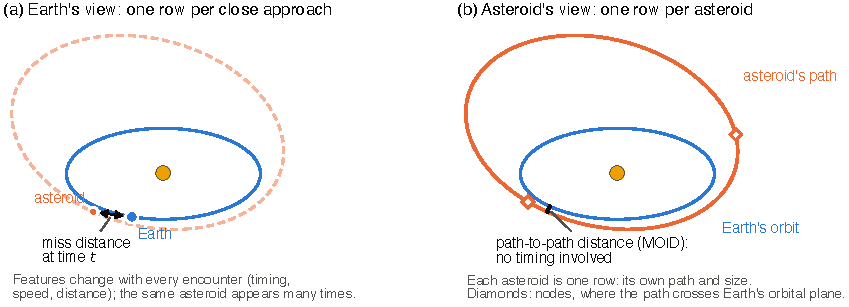
\includegraphics[width=\textwidth]{figures/fig1_concept.pdf}
\caption{Two ways to look at the same asteroid (illustrative orbit). (a) Earth's view: every close approach becomes a training row whose features depend on when the encounter happens. (b) Asteroid's view: one row per asteroid; hazard follows from the distance between the two paths, which involves no timing.}
\label{fig:concept}
\end{figure*}

Near-Earth asteroids (NEAs) whose orbits come within $0.05\au$ of Earth's orbit and whose absolute magnitude is $H \le 22$ (roughly 140\,m or larger) are designated potentially hazardous asteroids (PHAs)~\cite{cneos_groups}. The flag prioritises follow-up observation; whether an asteroid will actually strike Earth is a separate question answered by physics-based impact monitoring~\cite{milani2005,roa2021}.

A growing number of studies apply machine learning (ML) to the PHA flag~\cite{mclemore2022,malakouti2023,wang2023,surekha2024,nair2025,chandra2025,mondal2025,jacques2025} and report accuracies between 94\% and 99.7\% (Table~\ref{tab:literature}). Most of them build on NASA's Near Earth Object Web Service (NeoWs), in which each row is one close approach of an asteroid to Earth, or on Small-Body Database (SBDB) tables. We argue that this line of work has two problems.

\emph{Identity leakage.} An asteroid typically makes many recorded approaches, and its label is the same for all of them. A random split over rows therefore puts most test asteroids into the training set as well, a textbook form of leakage~\cite{kaufman2012,kapoor2023,roberts2017}.

\emph{A viewpoint mismatch.} The label is a property of the asteroid's \emph{path}: its minimum orbit intersection distance (MOID) with Earth's orbit and its size. Close-approach features are snapshots of single encounters at particular times. For a fixed pair of orbits, a miss distance can never be smaller than the MOID (Proposition~\ref{prop:miss}), so it bounds the quantity that defines the label but does not determine it.

We take the opposite view. Instead of looking at the asteroid from Earth at one moment, we look from the asteroid: each asteroid is one row, described only by its own heliocentric path and its size, and hazard is judged from the geometry of that path relative to Earth's orbit as a fixed curve. Where either body sits on its orbit at a given time never enters, so the timing of encounters cancels out (Fig.~\ref{fig:concept}). Because the path of a newly found asteroid is not known exactly, we also treat each path as a cloud of possible paths.

Our contributions are:
\begin{itemize}
\item A leakage audit of the Earth's-view benchmark on 306,590 JPL close approaches. Row-wise splits put 95.7\% of test rows next to their own asteroid in training; with grouped splits the best PHA-class F1 of the six prior-work models falls from 0.68 to 0.43, and no model we tried, including a convolutional network, GPBoost and a tuned random forest, exceeds 0.53.
\item An asteroid's-view formulation: a path kernel; an exact path-to-path distance checked against two-sided bounds and computed by two independent solvers that agree within $7\times10^{-10}\au$ (median deviation $1.0\times10^{-4}\au$ from JPL's MOID); closed-form bounds and a tangent-line kernel; Öpik encounter variables; and a dimensionless, training-free hazard index.
\item State-of-the-art results under leakage-free evaluation: 99.86\% accuracy and F1 0.989 on all 42,888 labelled NEAs without training; F1 0.99 instead of at most 0.53 on identical folds; no loss on post-2016 discoveries.
\item A decision layer with explicit abstention: a delta-method hazard probability on the signed distance, Monte Carlo where linearisation fails, and a branch-free decision law, machine-authored by integer program synthesis and verified on all $2^{32}$ inputs. With real orbit uncertainties it decides 99.43\% of NEAs, with no disagreement against the definition evaluated on JPL's MOID.
\item Complete proofs of every bound, equivalence and guarantee used (Appendix~\ref{app:proofs}), each confirmed numerically on the full catalogue (Appendix~\ref{app:verify}).
\item A path-cloud extension for uncertain orbits. In simulations built from the real error bars of short-arc NEAs, it is as accurate as the single-orbit rule (MCC within 0.002) and lowers the Brier score by 30--36\%.
\end{itemize}

\section{Related Work}

\subsection{Machine-learning classification of PHAs}
Table~\ref{tab:literature} summarises reported results. McLemore~\cite{mclemore2022} and Malakouti et al.~\cite{malakouti2023} train tree ensembles on NeoWs-derived tables; Wang~\cite{wang2023}, Surekha et al.~\cite{surekha2024} and Nair and Babu~\cite{nair2025} compare classifiers on similar data. Chandra~\cite{chandra2025} reports 99.7\% accuracy with a random forest under repeated stratified 10-fold cross-validation over 4,687 NeoWs records. Mondal et al.~\cite{mondal2025} combine tabular SBDB data with images and report 98.94\%. Jacques~\cite{jacques2025} models the full SBDB asteroid catalogue as a graph; with only 0.22\% hazardous objects, the reported 99\% accuracy coexists with a PHA-class F1 of 0.37 even though MOID is among the inputs. Several of these studies rebalance classes with SMOTE~\cite{chawla2002}. None of them reports an evaluation grouped by asteroid; in NeoWs-derived tables, where the same asteroid can appear in several close-approach records, this permits identity leakage. Hefele et al.~\cite{hefele2020} address a different task, training a neural network on simulated impactor orbits.

\begin{table*}[t]
\centering
\caption{Reported results of ML PHA classifiers, as published. Data, inputs and protocols differ, so the numbers are not directly comparable; Tables~\ref{tab:earthview} and~\ref{tab:samefolds} give like-for-like comparisons.}
\label{tab:literature}
\footnotesize
\setlength{\tabcolsep}{3.5pt}
\begin{tabularx}{\textwidth}{@{}>{\raggedright\arraybackslash}p{2.6cm}YYY>{\raggedright\arraybackslash}p{1.7cm}Y@{}}
\toprule
Work & Data & Inputs & Evaluation & Model & Best reported \\
\midrule
McLemore 2022~\cite{mclemore2022} & NeoWs table, 3,749 asteroids & orbit, size & grid-searched CV, held-out test & XGBoost & acc.\ 94.46\%, prec.\ 0.869, rec.\ 0.778 \\
Malakouti et al.\ 2023~\cite{malakouti2023} & NeoWs table (MOID among columns) & orbit, size, approach & random 80/10/10 split & random forest & bal.\ acc.\ 94\%, ROC-AUC 0.94 \\
Chandra 2025~\cite{chandra2025} & NeoWs table, 4,687 records & physical, orbital, approach & repeated stratified 10-fold over records & random forest & acc.\ 99.7\%, F2 0.987 \\
Mondal et al.\ 2025~\cite{mondal2025} & SBDB/NEO data, $>$30,000 asteroids, images & size, velocity, trajectory & random 80/20 split & hybrid ML/DL & acc.\ 98.94\% \\
Jacques 2025~\cite{jacques2025} & SBDB, 958,524 asteroids (0.22\% PHA) & orbit incl.\ MOID, physical & stratified 80/20, SMOTE & graph NN & acc.\ 99\%, F1 0.37, rec.\ 0.78 \\
\midrule
This work & SBDB, 42,888 NEAs & path and $H$ only & 5-fold over asteroids & training-free rule & acc.\ 99.86\%, F1 0.989, MCC 0.988 \\
This work & CAD, 306,590 approaches & path and $H$ only & asteroid-grouped 5-fold & training-free rule & acc.\ 99.79\%, F1 0.988, MCC 0.987 \\
This work & SBDB, 42,888 NEAs & path, $H$, element $\sigma$s & 5-fold over asteroids & decision law with abstention & decides 99.43\%; agrees with the definition on all decided \\
This work & Chandra's Kaggle table, 4,687 records~\cite{kaggle_nasa} & path and $H$ only & every record, no training & training-free rule & acc.\ 99.42\%, F1 0.982 (his model by asteroid: 99.42\%, 0.982) \\
\bottomrule
\end{tabularx}
\end{table*}

\subsection{Orbit geometry and impact monitoring}
The MOID is the minimum distance between two confocal Keplerian ellipses. Gronchi~\cite{gronchi2005} computes all critical points of the distance function algebraically; Wiśniowski and Rickman~\cite{wisniowski2013} give a fast geometric method; Hedo et al.~\cite{hedo2018,hedo2020} propose an efficient numerical method and asymptotic approximations. Öpik's theory~\cite{opik1976}, extended by Valsecchi et al.~\cite{valsecchi2003}, describes encounters through the encounter velocity implied by the orbit. Impact monitoring systems propagate orbit uncertainty to compute impact probabilities~\cite{milani2005,roa2021,milani_gronchi2009}; our path cloud borrows this idea for the PHA criterion.

\subsection{Evaluation pitfalls}
Leakage, where information about the test set reaches training, is a leading cause of irreproducible ML results in science~\cite{kaufman2012,kapoor2023}; grouped cross-validation is the standard remedy for repeated observations of the same unit~\cite{roberts2017}. With rare positives, accuracy is uninformative and the Matthews correlation coefficient (MCC) is preferable~\cite{chicco2020}.

\section{Data}

\subsection{Asteroid catalogue}
We queried the SBDB API~\cite{jpl_sbdb_api} on 11 November 2026 for all 43,025 near-Earth asteroids, retrieving osculating elements $(a, e, i, \Omega, \omega, M)$, $H$, element uncertainties, the orbit condition code, the first observation date, and JPL's Earth MOID and PHA flag. Of these, 42,888 have both an MOID and a flag (2,551 PHAs, 5.9\%); the 137 others are mostly unconstrained orbits (condition code 9).

\subsection{Close approaches (Earth's view)}
From the Close-Approach Data API~\cite{jpl_cad_api} we retrieved all approaches of NEOs to Earth within $0.5\au$ from 1910 to 2024, mirroring the NeoWs feed. Of 306,903 approaches, 306,590 belong to a labelled asteroid; they cover 36,817 asteroids, 8.74\% of rows are PHA approaches, and an asteroid contributes a median of 4 (mean 8.3, maximum 206) approaches. Each row receives the NeoWs features: $H$, the estimated diameter range for albedos 0.25 and 0.05, relative velocity and miss distance.

\subsection{The Kaggle NeoWs table}
For a same-file comparison with the strongest reported result we also use the public Kaggle table behind it~\cite{kaggle_nasa,chandra2025,malakouti2023}: 4,687 NeoWs records of 3,692 asteroids (16.1\% hazardous), with 40 columns including the orbital elements of April 2017 orbit solutions and an MOID. Of its asteroids, 751 appear in more than one record. Its labels contradict the definition applied to its own MOID and $H$ on 21 records of 15 asteroids, all with $21.9 \le H \le 22.6$.

\subsection{How exact is the label?}
Applying the definition to JPL's own MOID and $H$ reproduces JPL's flag for all but 49 asteroids (0.11\%). All 49 have $21.70 \le H \le 22.57$, i.e.\ they sit on the size boundary, where magnitude estimates are revised as observations accumulate. These cases cap the accuracy of any method that reproduces the definition at 99.886\%.

\section{The Asteroid's Point of View}

\subsection{Path kernel}
An asteroid's path is the curve
\begin{equation}
\mathbf{r}(f) = \frac{a(1-e^2)}{1+e\cos f}\left(\cos f\,\hat{\mathbf{P}} + \sin f\,\hat{\mathbf{Q}}\right), \quad f \in [0, 2\pi),
\label{eq:path}
\end{equation}
where $f$ is the true anomaly and the perifocal unit vectors in the ecliptic frame are
$\hat{\mathbf{P}} = (\cos\omega\cos\Omega - \sin\omega\sin\Omega\cos i,\ \cos\omega\sin\Omega + \sin\omega\cos\Omega\cos i,\ \sin\omega\sin i)$ and
$\hat{\mathbf{Q}} = (-\sin\omega\cos\Omega - \cos\omega\sin\Omega\cos i,\ -\sin\omega\sin\Omega + \cos\omega\cos\Omega\cos i,\ \cos\omega\sin i)$.
Earth's orbit is the fixed curve $\mathbf{E}(\lambda) = R(\lambda)(\cos\lambda, \sin\lambda, 0)$ with $R(\lambda) = p_\oplus/[1 + e_\oplus\cos(\lambda - \varpi_\oplus)]$, using the J2000 mean elements of the Earth--Moon barycentre~\cite{standish_approx} and neglecting its $1.5\times10^{-5}$\,deg inclination.

\subsection{Exact path-to-path distance}
The hazard-relevant geometry is the distance between the two curves,
\begin{equation}
\delta = \min_{f,\,\lambda}\ \lVert \mathbf{r}(f) - \mathbf{E}(\lambda) \rVert .
\label{eq:delta}
\end{equation}
It depends on $(a, e, i, \Omega, \omega)$ only. The mean anomaly and the epoch, i.e.\ where the asteroid and Earth are at any time, do not appear: the timing cancels (Proposition~\ref{prop:time}). For each $f$ we minimise over $\lambda$ with Newton's method started at the point's own longitude, which converges within four steps because $e_\oplus = 0.0167$. The outer minimisation samples 2048 values of $f$ and refines the four deepest local minima by golden-section search (48 steps). The cost is 0.28\,ms per asteroid in vectorised NumPy (12.1\,s for the whole catalogue on a laptop CPU). Against JPL's MOID, the median absolute difference is $1.0\times10^{-4}\au$, the 99th percentile $6.0\times10^{-4}\au$ and the correlation $r = 0.999997$ (Fig.~\ref{fig:geometry}a). The residual reflects our fixed J2000 Earth orbit versus JPL's epoch-specific one, and changes the PHA label of 9 of 42,888 asteroids. A second, independent solver parametrises Earth's orbit by its eccentric anomaly, solves the inner problem by Newton's method and refines the outer minima by Brent's method; it agrees with ours within $6.8\times10^{-10}\au$ on every asteroid (median $3\times10^{-15}\au$) and never changes a label. Each value is checked against the two-sided bounds of Section~\ref{sec:closed}, $\max(L_0, L_{\mathrm{lon}}) - \eta \le \delta \le \min(\delta_{\mathrm{node}}, U_{\mathrm{lon}}) + \eta$ with $\eta = 2\times10^{-8}\au$; all 42,888 values pass.

\begin{figure*}[t]
\centering
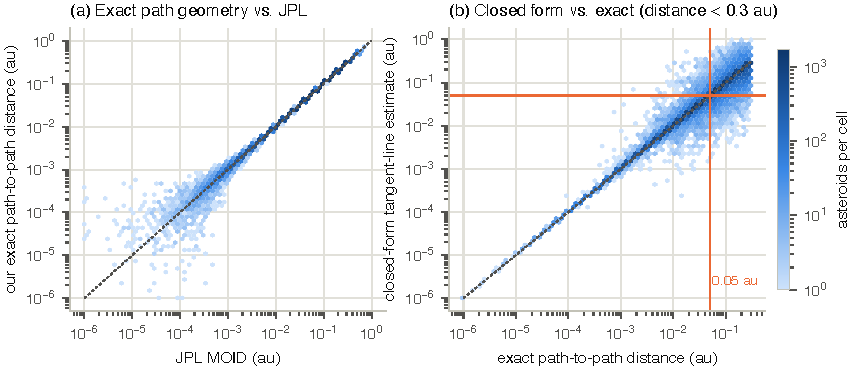
\includegraphics[width=\textwidth]{figures/fig4_geometry.pdf}
\caption{Geometry kernels against references, all 42,888 asteroids. (a) Exact path-to-path distance $\delta$ versus JPL's MOID. (b) Closed-form tangent-line estimate $\delta_{\mathrm{lin}}$ versus $\delta$ for $\delta < 0.3\au$; orange lines mark the $0.05\au$ threshold.}
\label{fig:geometry}
\end{figure*}

\subsection{Closed-form kernels and bounds}
\label{sec:closed}
Since $\lVert\mathbf{r}-\mathbf{E}\rVert \ge \bigl|\,|\mathbf{r}|-|\mathbf{E}|\,\bigr|$, the radial gap $L_0 = \max(0,\ q - Q_\oplus,\ q_\oplus - Q)$ is a lower bound on $\delta$ (Lemma~\ref{lem:radial}); $L_0 > 0.05\au$ settles Amors with $q > 1.067\au$ and Atiras with $Q < 0.933\au$. The path crosses the ecliptic at $f_+ = -\omega$ (ascending node, longitude $\Omega$) and $f_- = \pi - \omega$ (descending node, longitude $\Omega + \pi$), at heliocentric distances $r_\pm = a(1-e^2)/(1 \pm e\cos\omega)$. The radial gaps to Earth's orbit are $\Delta_+ = r_+ - R(\Omega)$ and $\Delta_- = r_- - R(\Omega + \pi)$, and the node gap $\delta_{\mathrm{node}} = \min(|\Delta_+|, |\Delta_-|)$ is an upper bound on $\delta$ (Lemma~\ref{lem:node}). Near a node we replace both paths by their tangent lines; the distance between these skew lines is (Lemma~\ref{lem:lin})
\begin{equation}
\delta_{\mathrm{lin},\pm} = \frac{|\Delta_\pm|\,\sin i}{\sqrt{\sin^2 i\,(1 + k_\oplus^2) + (k_a - k_\oplus\cos i)^2}},
\label{eq:lin}
\end{equation}
where $k_a = e\sin f_\pm / (1 + e\cos f_\pm)$ and $k_\oplus = e_\oplus\sin\psi/(1 + e_\oplus\cos\psi)$, with $\psi$ the node longitude minus $\varpi_\oplus$, are the ratios of radial to transverse velocity of the asteroid and of Earth at the node. We use $\delta_{\mathrm{lin}} = \min(\delta_{\mathrm{lin},+}, \delta_{\mathrm{lin},-})$. Eq.~\eqref{eq:lin} is exact to first order when both paths are nearly straight across the gap, which is the regime that matters for $\delta \le 0.05\au$; it degrades at very low inclination, where the nodes are ill-defined. First-order approximations of this kind are classical (see~\cite{hedo2018,hedo2020} and references therein); we use it as a feature and as a closed-form classifier. Finally, for a point with cylindrical coordinates $(\rho, \lambda, z)$ and $g = \rho - R(\lambda)$, its distance $d$ to Earth's orbit satisfies $z^2 + \kappa g^2 \le d^2 \le z^2 + g^2$, with $\kappa = c/(c + K_\oplus^2)$, $c = 4\rho\,q_\oplus/\pi^2$ and $K_\oplus = p_\oplus e_\oplus/(1 - e_\oplus)^2 \ge \max_\lambda |R'(\lambda)|$. Minimising both sides over $f$ gives a same-longitude bracket $L_{\mathrm{lon}} \le \delta \le U_{\mathrm{lon}}$ (Lemma~\ref{lem:bracket}, Corollary~\ref{cor:bracket}), which is exact for a circular Earth orbit and at most $2.1\times10^{-5}\au$ wide wherever $\delta \le 0.05\au$.

\subsection{Öpik encounter variables}
In units of Earth's orbital radius and speed, the Tisserand parameter with respect to Earth, $T_\oplus = 1/a + 2\sqrt{a(1-e^2)}\cos i$, gives the encounter speed $U = \sqrt{3 - T_\oplus}$ and its direction, $\cos\theta = (1 - U^2 - 1/a)/(2U)$~\cite{opik1976,valsecchi2003}. They describe any encounter the path allows, again without reference to time.

\subsection{A dimensionless hazard index}
Each asteroid is assigned the value
\begin{equation}
\Phi = \max\!\left( \frac{\delta}{\delta_0},\ 10^{(H - H_0)/5} \right), \qquad \delta_0 = 0.05\au,\ H_0 = 22 .
\label{eq:phi}
\end{equation}
Because diameter scales as $D \propto p_V^{-1/2}\,10^{-H/5}$~\cite{pravec2007}, the second term equals $D_0/D$ for equal albedo, so both terms are dimensionless ratios of the asteroid's own path and size to the thresholds of the definition. An asteroid is a PHA exactly when $\Phi \le 1$ (Proposition~\ref{prop:phi}), and $s = -\ln\Phi$ ranks asteroids continuously (used for ROC analysis). With $\delta$ from \eqref{eq:delta} this is a training-free classifier; with $\delta_{\mathrm{lin}}$ from \eqref{eq:lin} it is a closed-form one.

\subsection{Hazard probability under orbit uncertainty}
\label{sec:prob}
Let $F$ denote the standard normal distribution function. At the minimising pair, let $\boldsymbol{\Delta} = \mathbf{r}(f^*) - \mathbf{E}(\lambda^*)$ and let $\boldsymbol{\tau}$, $\boldsymbol{\tau}_\oplus$ be the two tangents. The signed distance $\tilde d = \hat{\mathbf{n}}\cdot\boldsymbol{\Delta}$ with $\hat{\mathbf{n}} = \boldsymbol{\tau}_\oplus\times\boldsymbol{\tau}/\lVert\boldsymbol{\tau}_\oplus\times\boldsymbol{\tau}\rVert$ equals $\pm\delta$ and stays smooth through orbit crossings~\cite{gronchi2007} (Proposition~\ref{prop:grad}). By the envelope theorem, $\partial\tilde d/\partial x_k = \hat{\mathbf{n}}\cdot\partial\mathbf{r}/\partial x_k$ at $f^*$, so with $\Sigma = \mathrm{diag}(\sigma_a^2, \sigma_e^2, \sigma_i^2, \sigma_\Omega^2, \sigma_\omega^2)$ the spread is $s^2 = \nabla\tilde d^{\top}\Sigma\,\nabla\tilde d$ and
\begin{equation}
P_{\mathrm{lin}} = F\!\left(\frac{\delta_0 - \tilde d}{s}\right) - F\!\left(\frac{-\delta_0 - \tilde d}{s}\right).
\label{eq:plin}
\end{equation}
The linearisation is trusted only if $s \le 0.01\au$, the runner-up local minimum lies at least $5s$ above $\delta$, and the tangents are not nearly parallel; otherwise we use the path cloud below. A score with a fitted offset, $S = \mathbf{1}[H \le H_0]\,[F((\delta_0 + \beta - \tilde d)/s_{\mathrm{eff}}) - F((-\delta_0 - \beta - \tilde d)/s_{\mathrm{eff}})]$ with $s_{\mathrm{eff}} = \sqrt{s^2 + w^2}$, lets a systematic offset $\beta$ between our Earth curve and JPL's, and residual scatter $w$, be fitted by maximum likelihood on training labels; with $\beta = w = s = 0$ it is the rule $\Phi \le 1$.

When an orbit is uncertain, the path is a cloud rather than a curve. We draw $N$ clones $\mathbf{x}^{(n)} \sim \mathcal{N}(\hat{\mathbf{x}}, \Sigma)$ of the elements, with $\Sigma$ diagonal from the 1$\sigma$ uncertainties when no covariance is available, and estimate
\begin{equation}
P_{\mathrm{haz}} = \frac{1}{N}\sum_{n=1}^{N} \mathbf{1}\!\left[ \Phi(\mathbf{x}^{(n)}, H) \le 1 \right].
\label{eq:cloud}
\end{equation}
An asteroid is flagged when $P_{\mathrm{haz}} \ge \tau$, with $\tau$ chosen on training data only. Under a flat prior on the true orbit, \eqref{eq:cloud} is a Monte Carlo estimate of the posterior probability that the asteroid meets the definition~\cite{milani_gronchi2009} (Proposition~\ref{prop:prob}); inside the decision procedure we use 4,000 draws and a 95\% Wilson interval~\cite{wilson1927}.

\subsection{A decision law with abstention}
\label{sec:law}
The kernels produce bounds, certificates and probabilities; a fixed law turns them into an act. It reads only a 9-bit situation word, never an orbit, a magnitude or a time: whether the input is valid; whether $H > 22$; the certificate state (open, far with $L_0 > \delta_0$, near with $\delta_{\mathrm{node}} \le \delta_0$, exact far, exact near, or failed); the uncertainty state; and the probability band (sure in, $P \ge 1 - \alpha$; middle; sure out, $P \le \alpha$; with $\alpha = F(-3)$). It returns one of ten acts: run a kernel (exact distance, delta method, sampling), decide (PHA; not a PHA by size; not a PHA by geometry), abstain with follow-up (observe a nominal PHA, or a nominal non-PHA, whose label could flip within the uncertainty), or refer to a human (invalid input or failed check). Every act changes the word, so the procedure ends within six steps, and every decided class agrees with its certificate (Theorem~\ref{thm:law}). The law is a branch-free integer program, machine-authored by integer program synthesis from its truth table. We verified it against an independent transcription of its specification on all $2^{32}$ 32-bit inputs with no mismatch; compiled with clang at \texttt{-O2}, it is 60 arm64 instructions without a branch. A systematic difference $s_{\mathrm{sys}}$ between our Earth curve and JPL's can be added in quadrature to every spread; a cheap certificate is then accepted only if it clears $\delta_0$ by $3s_{\mathrm{sys}}$.

\subsection{Learned asteroid's-view models}
We also train classifiers on three feature sets: \emph{path} ($a, e, i$, $\sin$ and $\cos$ of $\Omega$ and $\omega$, $q$, $Q$, $H$); \emph{path + kernels}, which adds $r_\pm$, $\Delta_\pm$, $\delta_{\mathrm{node}}$, $\delta_{\mathrm{lin},\pm}$, $\delta_{\mathrm{lin}}$, $T_\oplus$, $U$ and $\cos\theta$; and \emph{path + kernels + exact}, which adds $\delta$. None of them uses JPL's MOID or PHA columns, close-approach data, or Earth's position at any time.

\section{Experimental Setup}

\begin{figure*}[t]
\centering
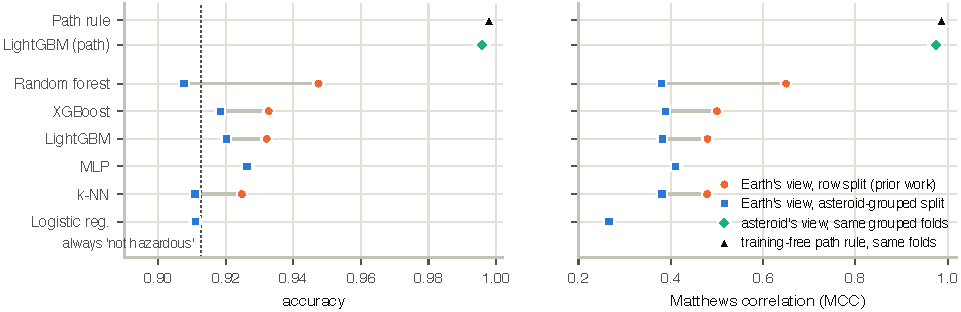
\includegraphics[width=\textwidth]{figures/fig3_leakage.pdf}
\caption{Leakage audit on 306,590 approaches. Circles: Earth's-view models under the row split used in prior work; squares: the same models when all approaches of an asteroid share a fold. Diamond and triangle: the asteroid's view on the same grouped folds. Dashed line: always predicting ``not hazardous''.}
\label{fig:leakage}
\end{figure*}

\begin{figure*}[t]
\centering
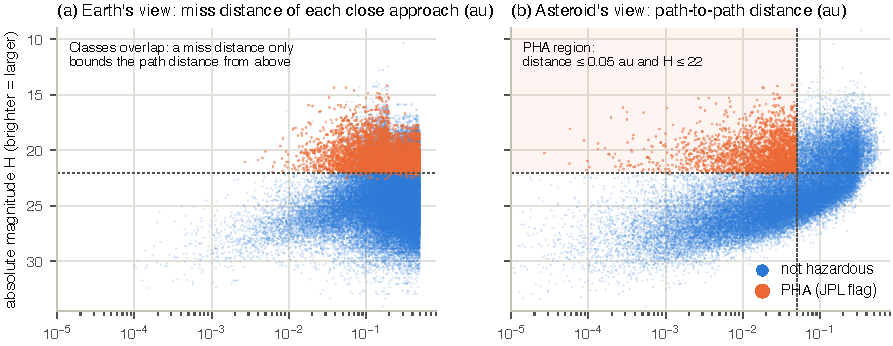
\includegraphics[width=\textwidth]{figures/fig2_viewpoints.pdf}
\caption{The same catalogue from both viewpoints (60,000 sampled approaches in (a); all 42,888 asteroids in (b)). (a) Against miss distance, PHAs and other asteroids overlap, because a miss distance only bounds the path distance from above. (b) Against the path-to-path distance $\delta$, the PHA label becomes the rectangle $\delta \le 0.05\au$, $H \le 22$.}
\label{fig:viewpoints}
\end{figure*}

\subsection{Protocols}
(i)~\emph{Earth's view, row split:} stratified 5-fold cross-validation over approach rows, as in prior work. (ii)~\emph{Earth's view, grouped:} stratified group 5-fold, keeping all approaches of an asteroid in one fold. (iii)~\emph{Asteroid's view:} stratified 5-fold over asteroids, one row each. (iv)~\emph{Same folds:} asteroid's-view models are trained on the training asteroids of (ii) and their predictions are applied to every approach of each test asteroid, so the scores are computed on exactly the rows of (ii). (v)~\emph{Temporal:} train on the 15,071 asteroids first observed before 2016 (1,869 PHAs), test on the 27,817 discovered since (682 PHAs). (vi)~\emph{Reference:} orbital elements plus JPL's MOID column, the setting of SBDB- and NeoWs-based studies~\cite{malakouti2023,jacques2025}; it uses the quantity that defines the label and is reported for context only. (vii)~\emph{Decision procedure:} every NEA is processed with its real 1$\sigma$ element uncertainties, first as specified ($s_{\mathrm{sys}} = 0$), then with $s_{\mathrm{sys}}$ equal to the root-mean-square difference between our distance and JPL's MOID on the training asteroids of a 5-fold split by asteroid; JPL's MOID never enters a test decision. The score offsets $\beta$ and $w$ are fitted on the same training folds.

\subsection{Models and metrics}
We use logistic regression, $k$-nearest neighbours, random forests~\cite{breiman2001}, XGBoost~\cite{chen2016}, LightGBM~\cite{ke2017} and a multilayer perceptron, implemented with scikit-learn~\cite{pedregosa2011}. For a comparison with three further model families we also train a one-dimensional convolutional network over the standardised feature vector (two convolution layers and a dense head, implemented in PyTorch~\cite{paszke2019}, with early stopping on 10\% of the training rows), GPBoost~\cite{sigrist2022}, which adds a random effect per asteroid to tree boosting, and a random forest tuned for F1 by randomised search inside the training folds, with the inner splits grouped by asteroid whenever the outer split is. Hyperparameters are otherwise fixed in advance, and none is tuned on test folds; the decision threshold is 0.5 and the random seed is fixed. We report accuracy, balanced accuracy, precision, recall and F1 for the PHA class, MCC~\cite{chicco2020} and ROC-AUC, plus the Brier score for probabilistic outputs. PHAs are rare (5.9\% of NEAs, 8.7\% of approach rows), so always predicting ``not hazardous'' already scores 91.3\% accuracy on approach rows.

\subsection{Uncertainty simulation}
Ground truth consists of the 11,054 NEAs with well-determined orbits (condition code 0--2; 2,039 PHAs), labelled by applying the definition to $\delta$ of their true orbits. To mimic orbits that are not yet well known, each true orbit receives the element uncertainties of a randomly drawn NEA from one of two orbit-quality classes: moderately determined (condition code 5--7; 17,690 profiles; median observed arc 20 days) or short-arc (condition code 8--9; 12,474 profiles; median arc 6 days). The uncertainties are scaled by $\times0.25$ to $\times2$, and the orbit is perturbed by Gaussian noise of that size; for each element, at most 0.3\% of profiles exceed generous caps and are clipped. Every method sees only the perturbed orbit, its uncertainties and $H$: the PHA rule applied to the single perturbed orbit (exact or closed form), LightGBM trained on the perturbed orbits, uncertainties and kernels, the path cloud \eqref{eq:cloud} with $N = 48$, and LightGBM with $P_{\mathrm{haz}}$ as an extra feature. We use 5-fold cross-validation over the truth set.

\begin{table}[t]
\centering
\footnotesize
\caption{Earth's-view benchmark on 306,590 JPL close approaches (36,817 asteroids). Row split: stratified 5-fold over rows, as in prior work (95.7\% of test rows belong to an asteroid seen in training). Grouped: all approaches of an asteroid share a fold. Means over 5 folds.}
\label{tab:earthview}
\setlength{\tabcolsep}{2.4pt}
\begin{tabular}{@{}lcccccc@{}}
\toprule
 & \multicolumn{3}{c}{Row split (leaky)} & \multicolumn{3}{c}{Grouped (honest)} \\
\cmidrule(lr){2-4}\cmidrule(l){5-7}
Model & Acc.\,\% & F1 & MCC & Acc.\,\% & F1 & MCC \\
\midrule
Logistic regression & 91.12 & 0.279 & 0.268 & 91.09 & 0.277 & 0.266 \\
$k$-NN ($k{=}5$) & 92.48 & 0.514 & 0.479 & 91.09 & 0.425 & 0.381 \\
MLP & 92.67 & 0.400 & 0.413 & \textbf{92.63} & 0.398 & \textbf{0.410} \\
LightGBM & 93.21 & 0.479 & 0.480 & 92.02 & 0.397 & 0.382 \\
XGBoost & 93.27 & 0.513 & 0.500 & 91.84 & 0.414 & 0.388 \\
Random forest & \textbf{94.74} & \textbf{0.676} & \textbf{0.650} & 90.76 & \textbf{0.428} & 0.380 \\
\midrule
Always ``not hazardous'' & 91.26 & 0.000 & 0.000 & 91.26 & 0.000 & 0.000 \\
\bottomrule
\end{tabular}
\end{table}


\section{Results}

\begin{table*}[t]
\centering
\footnotesize
\caption{Asteroid's-view results on all 42,888 labelled near-Earth asteroids: stratified 5-fold cross-validation over asteroids (one row per asteroid, so no asteroid is in both training and test data). Means over folds; across all rows, fold standard deviations are at most 0.17 percentage points for accuracy and 0.016 for F1 and MCC. Best non-reference value per column in bold. $^\dagger$Rows marked with a dagger use JPL's own MOID column, i.e.\ the quantity that defines the label.}
\label{tab:asteroidview}
\begin{tabular}{@{}lcccccc@{}}
\toprule
Method (features) & Accuracy\,\% & Bal.\ acc.\,\% & Precision & Recall & F1 & MCC \\
\midrule
\multicolumn{7}{@{}l}{\emph{Training-free, asteroid's view}} \\
Path rule, exact geometry (ours) & \textbf{99.86} & 99.23 & 0.992 & 0.985 & \textbf{0.989} & \textbf{0.988} \\
Path rule, tangent-line closed form (ours) & 99.26 & 96.74 & 0.937 & 0.939 & 0.938 & 0.934 \\
Path rule, node gap (upper bound) & 97.16 & 76.31 & \textbf{0.993} & 0.526 & 0.688 & 0.712 \\
\midrule
\multicolumn{7}{@{}l}{\emph{Learned, asteroid's view}} \\
LightGBM (path) & 98.38 & 92.07 & 0.875 & 0.849 & 0.862 & 0.853 \\
XGBoost (path) & 98.38 & 92.29 & 0.871 & 0.854 & 0.862 & 0.854 \\
Random forest (path + kernels) & 99.58 & 97.48 & 0.978 & 0.951 & 0.964 & 0.962 \\
XGBoost (path + kernels) & 99.69 & 98.35 & 0.979 & 0.968 & 0.974 & 0.972 \\
LightGBM (path + kernels) & 99.71 & 98.52 & 0.979 & 0.972 & 0.976 & 0.974 \\
Random forest (path + kernels + exact) & 99.85 & \textbf{99.28} & 0.989 & \textbf{0.986} & 0.988 & 0.987 \\
LightGBM (path + kernels + exact) & 99.82 & 99.04 & 0.988 & 0.982 & 0.985 & 0.984 \\
\midrule
\multicolumn{7}{@{}l}{\emph{Reference: uses JPL's MOID column$^\dagger$}} \\
Definition on JPL MOID$^\dagger$ & 99.89 & 99.35 & 0.993 & 0.987 & 0.990 & 0.990 \\
Random forest (orbit + JPL MOID) & 99.87 & 99.34 & 0.991 & 0.987 & 0.989 & 0.988 \\
LightGBM (orbit + JPL MOID) & 99.82 & 99.17 & 0.985 & 0.984 & 0.985 & 0.984 \\
\bottomrule
\end{tabular}
\end{table*}

\begin{table}[t]
\centering
\footnotesize
\caption{Head-to-head on identical asteroid-grouped folds, scored per close-approach row (306,590 rows). Asteroid's-view models are trained on the training asteroids' paths and their prediction is applied to every approach of each test asteroid.}
\label{tab:samefolds}
\setlength{\tabcolsep}{2.2pt}
\begin{tabular}{@{}lcccc@{}}
\toprule
Method & Acc.\,\% & F1 & MCC & AUC \\
\midrule
Earth: MLP & 92.63 & 0.398 & 0.410 & 0.9408 \\
Earth: XGBoost & 91.84 & 0.414 & 0.388 & 0.9326 \\
Earth: Random forest & 90.76 & 0.428 & 0.380 & 0.9230 \\
\midrule
Asteroid: rule, exact geometry & \textbf{99.79} & \textbf{0.988} & \textbf{0.987} & \textbf{0.9998} \\
Asteroid: rule, closed form & 99.12 & 0.949 & 0.944 & 0.9908 \\
Asteroid: LightGBM (path) & 96.95 & 0.822 & 0.806 & 0.9916 \\
Asteroid: LightGBM (path + kernels) & 99.59 & 0.976 & 0.974 & 0.9994 \\
Asteroid: XGBoost (path + kernels) & 99.55 & 0.974 & 0.971 & 0.9996 \\
\bottomrule
\end{tabular}
\end{table}


\subsection{Leakage inflates Earth's-view scores}
Table~\ref{tab:earthview} and Fig.~\ref{fig:leakage} reproduce the prior-work protocol. With row splits, 95.7\% of test rows belong to an asteroid seen in training, exactly as Proposition~\ref{prop:leak} predicts from the data's multiplicities, and a random forest reaches 94.74\% accuracy and F1 0.676, in line with published Earth's-view results~\cite{mclemore2022,malakouti2023}. With asteroid-grouped splits the same model falls to 90.76\% accuracy and F1 0.428. The best grouped accuracy is 92.63\% (MLP), only 1.4 points above the trivial baseline, and the best MCC in Table~\ref{tab:earthview} is 0.41. Models that can memorise asteroids lose the most: $H$ repeats across an asteroid's approaches and acts as an identifier.

\subsection{Why the viewpoint matters}
Fig.~\ref{fig:viewpoints} shows the reason. Seen from Earth, a PHA can pass at a large distance in any given encounter, so the classes overlap in every snapshot. Seen from the asteroid, the label is a rectangle in the plane of path distance and size.

\subsection{The asteroid's view reaches the ceiling}
Table~\ref{tab:asteroidview} gives the asteroid's-view results. The training-free path rule reaches 99.865\% accuracy, F1 0.989 and MCC 0.988, about 0.02 percentage points below the definition applied to JPL's own MOID (99.886\%), which is the ceiling set by the inconsistent flags. The closed-form tangent-line rule reaches 99.26\% (F1 0.938) without any optimisation. Learned models trained on the raw path reach 98.38\% (F1 0.862); the closed-form kernels lift LightGBM to 99.71\% (F1 0.976), because they encode geometry that trees find hard to assemble from raw angles. Giving the learner the exact distance $\delta$ lets it approach, but not beat, the rule. Even the reference setting that hands ML JPL's MOID column only matches the training-free rule (99.87\% against 99.86\%, F1 0.989 for both), well within the fold-to-fold spread.

\subsection{Head-to-head on identical folds}
On exactly the rows and folds of the grouped Earth's-view benchmark (Table~\ref{tab:samefolds}), the asteroid's view raises accuracy from 92.63\% to 99.79\%, F1 from 0.428 to 0.988 and MCC from 0.410 to 0.987. A learned model on the path and kernels reaches F1 0.976.

\subsection{Generalization to new discoveries}
Recent discoveries are smaller and fainter, and only 2.5\% of them are PHAs. Trained on asteroids found before 2016 and tested on later ones (Table~\ref{tab:temporal}), the path rule keeps F1 0.988, and LightGBM on path and kernels reaches F1 0.972; on the raw path alone it drops to 0.835.

\begin{table}[t]
\centering
\footnotesize
\caption{Temporal generalization: train on the 15,071 asteroids first observed before 2016, test on the 27,817 discovered since (2.5\% PHAs). RF: random forest; k: geometry kernels. $^\dagger$Uses JPL's MOID column.}
\label{tab:temporal}
\setlength{\tabcolsep}{2pt}
\begin{tabular}{@{}lccccc@{}}
\toprule
Method (features) & Acc.\,\% & Prec. & Rec. & F1 & MCC \\
\midrule
Rule: exact geometry & \textbf{99.94} & \textbf{0.990} & 0.987 & \textbf{0.988} & \textbf{0.988} \\
Rule: closed form & 99.72 & 0.944 & 0.943 & 0.944 & 0.942 \\
LightGBM (path) & 99.18 & 0.822 & 0.848 & 0.835 & 0.831 \\
LightGBM (path+k) & 99.86 & 0.967 & 0.977 & 0.972 & 0.971 \\
XGBoost (path+k) & 99.86 & 0.973 & 0.969 & 0.971 & 0.971 \\
RF (path+k+exact) & 99.93 & 0.981 & \textbf{0.991} & 0.986 & 0.986 \\
\midrule
Definition on JPL MOID$^\dagger$ & 99.95 & 0.991 & 0.990 & 0.990 & 0.990 \\
RF (orbit+JPL MOID)$^\dagger$ & 99.94 & 0.980 & 0.994 & 0.987 & 0.987 \\
\bottomrule
\end{tabular}
\end{table}


\subsection{Certified screening and abstention on the real catalogue}
All 42,888 exact distances pass their bound check, at a median 0.66\,ms per asteroid. The closed-form bounds alone settle 51.1\% of the 11,761 bright NEAs ($H \le 22$): 39.6\% have $L_0 > 0.05\au$ and 11.5\% have $\delta_{\mathrm{node}} \le 0.05\au$, with no conflict with JPL's MOID in either group. Fitting the score offset on training folds gives $\hat\beta = (-1.1 \pm 2.9)\times10^{-4}\au$, consistent with zero, and does not improve agreement (99.860\% against 99.865\%); the remaining disagreements are not an offset in the distance.

\begin{table}[t]
\centering
\footnotesize
\caption{The decision procedure on all 42,888 labelled NEAs with their real 1$\sigma$ element uncertainties. Left: the law as specified; right: with the Earth-curve systematic $s_{\mathrm{sys}} = 2.4\times10^{-4}$\,au measured on the training folds (5-fold, by asteroid). Agreement is over decided asteroids; ``observe'' marks asteroids whose label could flip within their uncertainty.}
\label{tab:decision}
\setlength{\tabcolsep}{3pt}
\begin{tabular}{@{}lrr@{}}
\toprule
Act & $s_{\mathrm{sys}} = 0$ & measured $s_{\mathrm{sys}}$ \\
\midrule
PHA & 2,496 & 2,466 \\
Not PHA: geometry & 9,077 & 9,051 \\
Not PHA: size ($H > 22$) & 31,127 & 31,127 \\
Observe, nominal PHA & 37 & 67 \\
Observe, nominal non-PHA & 151 & 177 \\
Human referral & 0 & 0 \\
\midrule
Decided (coverage) & 99.56\% & 99.43\% \\
Agrees with JPL flag & 99.869\% & 99.887\% \\
\quad disagreements & 56 & 48 \\
\quad flag contradicts definition & 48 & 48 \\
Agrees with definition on JPL MOID & 99.981\% & 100.000\% \\
\bottomrule
\end{tabular}
\end{table}


Table~\ref{tab:decision} shows the decision procedure with each asteroid's real uncertainties. As specified, it refers no asteroid to a human, decides 99.56\% and flags 188 (0.44\%) for follow-up, 173 of them with short-arc orbits (condition code 8--9). Its 56 disagreements with JPL's flag are of two kinds: 48 flags that contradict JPL's own definition, all at the $H = 22$ boundary, and 8 asteroids whose distance lies within $5.1\times10^{-4}\au$ of the threshold, where our Earth curve and JPL's differ. Adding the measured systematic $s_{\mathrm{sys}} = 2.4\times10^{-4}\au$ moves those 8 to the follow-up class. The procedure then decides 99.43\% of NEAs, agrees with the definition evaluated on JPL's MOID for every one of them, and disagrees with JPL's flag only where the flag contradicts that definition. On the 32 real orbits whose linearised probability lies between 0.01 and 0.99, the delta method \eqref{eq:plin} falls inside the Monte Carlo 95\% interval ($\pm0.01$) in every case, with a median difference of 0.005.

\subsection{Uncertain orbits}
Table~\ref{tab:uncertainty} and Fig.~\ref{fig:uncertainty} show the simulation. With moderately determined orbits (condition code 5--7) the error bars are small: at the real error level, the PHA rule applied to the perturbed orbit mislabels only 0.11\% of asteroids and remains the best hard classifier (MCC 0.996). The path cloud gives up a little of that (MCC 0.994) in exchange for better probabilities, with a lower Brier score at three of the four uncertainty levels and ROC-AUC of at least 0.9999. With short-arc orbits (condition code 8--9, median arc 6 days) the single-orbit rule mislabels 1.54\% of asteroids. Here the path cloud matches it on hard decisions (98.46\% accuracy and MCC 0.949 for both) and lowers the Brier score by 32\% (0.0105 instead of 0.0154). Across the four uncertainty levels the reduction is 30--36\%, and at $\times0.5$ and $\times2$ the cloud also has the highest MCC. LightGBM trained on the same orbits, uncertainties and kernels never beats the single-orbit rule; with the cloud probability as an extra feature it does so once, by less than 0.001 in MCC, at the smallest short-arc uncertainty. The value of the path cloud is therefore calibrated hazard probabilities for poorly known orbits, which is what follow-up prioritisation needs, rather than higher accuracy for well-known ones.

\begin{table*}[t]
\centering
\footnotesize
\caption{Hazard classification from uncertain orbits (simulation, real error bars $\times1$). Truth: 11,054 well-determined NEAs (2,039 PHAs). Each true orbit is perturbed with the element uncertainties of a randomly drawn NEA of the given orbit-quality class (17,690 and 12,474 profiles); methods see only the perturbed orbit, its 1$\sigma$ uncertainties and $H$. Applied to the perturbed orbit, the PHA rule mislabels 0.11\% and 1.54\% of asteroids, respectively. Path cloud: 48 clones per asteroid. Means over 5 folds.}
\label{tab:uncertainty}
\begin{tabular}{@{}lcccccccc@{}}
\toprule
 & \multicolumn{4}{c}{Condition code 5--7} & \multicolumn{4}{c}{Condition code 8--9 (short arcs)} \\
\cmidrule(lr){2-5}\cmidrule(l){6-9}
Method & Acc.\,\% & MCC & ROC-AUC & Brier & Acc.\,\% & MCC & ROC-AUC & Brier \\
\midrule
Single orbit, exact rule & \textbf{99.89} & \textbf{0.996} & 0.9978 & 0.0011 & \textbf{98.46} & \textbf{0.949} & 0.9741 & 0.0154 \\
Single orbit, closed form & 98.12 & 0.938 & 0.9687 & 0.0188 & 96.93 & 0.898 & 0.9476 & 0.0307 \\
LightGBM (orbit, $\sigma$s, kernels) & 99.79 & 0.993 & 0.9998 & 0.0018 & 98.31 & 0.944 & 0.9981 & 0.0150 \\
Path cloud (ours) & 99.81 & 0.994 & \textbf{1.0000} & \textbf{0.0009} & \textbf{98.46} & \textbf{0.949} & \textbf{0.9989} & \textbf{0.0105} \\
LightGBM + path cloud (ours) & 99.79 & 0.993 & 0.9999 & 0.0019 & 98.37 & 0.946 & 0.9985 & 0.0146 \\
\bottomrule
\end{tabular}
\end{table*}


\begin{figure*}[t]
\centering
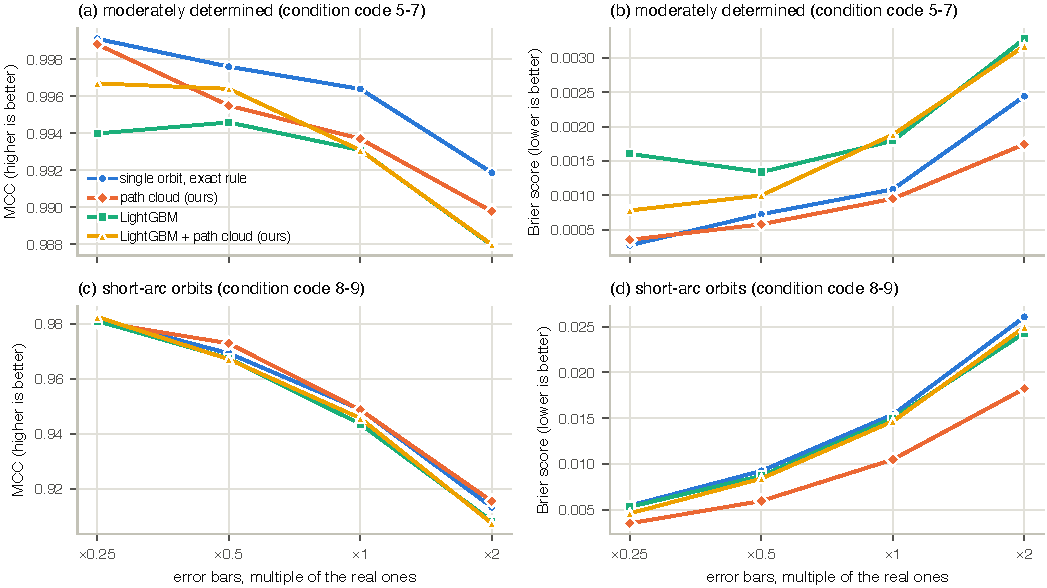
\includegraphics[width=\textwidth]{figures/fig5_uncertainty.pdf}
\caption{Hazard classification from uncertain orbits (simulation; error bars scaled from the real ones). Top: uncertainties of moderately determined NEAs; bottom: short-arc NEAs. Left: MCC of the hard decisions; right: Brier score of the predicted probabilities (for the single-orbit rule, its error rate). The closed-form single-orbit rule is listed in Table~\ref{tab:uncertainty}.}
\label{fig:uncertainty}
\end{figure*}

\subsection{Same-file comparison with the strongest reported result}
The highest accuracy we found in the literature is 99.7\%, obtained with a random forest under record-level cross-validation on the Kaggle NeoWs table~\cite{chandra2025}; on the full SBDB catalogue the best reported PHA-class F1 is 0.37~\cite{jacques2025}. Table~\ref{tab:kaggle} reruns the strongest result on its own file. With the record-level protocol, a random forest on every numeric column reaches 99.62\%, close to the reported 99.7\%, and above the 99.55\% that the definition itself scores on this table. That is possible only by learning labels that contradict the definition. When such a record's asteroid also had a record in the training folds, the forest reproduced its inconsistent label in 23 of 31 cases; when it had not, in 4 of 32. Split by asteroid, the same forest falls to 99.42\% (F1 0.982), the same accuracy to two decimals as our training-free rule (99.42\%, F1 0.982, MCC 0.979), which never reads the table's MOID column. Of the rule's 27 errors, 21 are records whose label contradicts the definition and 6 lie at the threshold, where our distance and the table's 2017 MOID differ. On this file the asteroid's view therefore ties the strongest model under honest evaluation, and the reported margin comes from identity leakage. On the complete current catalogue (Table~\ref{tab:literature}), the training-free rule reaches 99.86\% accuracy and F1 0.989.

\begin{table}[t]
\centering
\footnotesize
\caption{Same-file comparison on the Kaggle NeoWs table behind the highest reported accuracy~\cite{kaggle_nasa,chandra2025}: 4,687 records of 3,692 asteroids, 16.1\% hazardous. Random-forest rows use every numeric column, including the table's MOID; repeated stratified 10-fold $\times$3. Our rule computes the distance from the table's orbital elements and never reads its MOID column. RF: random forest; k: geometry kernels. $^\dagger$The ceiling for any method that follows the definition.}
\label{tab:kaggle}
\setlength{\tabcolsep}{2.2pt}
\begin{tabular}{@{}lcccc@{}}
\toprule
Method & Acc.\,\% & F1 & F2 & MCC \\
Reported~\cite{chandra2025}, RF by record & 99.7 & -- & 0.987 & -- \\
\midrule
RF by record (reproduced) & 99.62 & 0.988 & 0.986 & 0.986 \\
RF by asteroid & 99.42 & 0.982 & 0.977 & 0.978 \\
Training-free path rule (ours) & 99.42 & 0.982 & 0.980 & 0.979 \\
LightGBM, path+k, by asteroid (ours) & 98.98 & 0.968 & 0.964 & 0.962 \\
\midrule
Definition on the table's MOID$^\dagger$ & 99.55 & 0.986 & 0.985 & 0.983 \\
\bottomrule
\end{tabular}
\end{table}


\subsection{Three further model families}
Table~\ref{tab:sheet} adds a convolutional network, GPBoost and a tuned random forest. On the 306,590 approaches they use the CAD table's own columns (miss distance with its $3\sigma$ range, relative and asymptotic speed, and $H$), with JPL's PHA flag as the label and the folds of Table~\ref{tab:earthview}. Under the row split, GPBoost's random effect per asteroid memorises the asteroids it has already seen and reaches 99.90\% accuracy (F1 0.994); on new asteroids that effect is zero, and the model never predicts a PHA (F1 0.000, ROC-AUC 0.919). On the grouped folds the three models reach 92.61\%, 91.26\% and 87.00\% accuracy and at most F1 0.527, against 99.79\% and F1 0.988 for the training-free rule. The same holds on two small JPL tables. On 33 Earth approaches within $0.05\au$ between September and November 2026, two of them by PHAs, the rule labels every object correctly, while the three models, trained by leave-one-out, find neither PHA. On the Sentry impact-risk list~\cite{jpl_sentry_api}, where 2,241 of the 2,242 objects have an absolute magnitude in JPL's catalogue (15 PHAs), the rule is again exact and the best model reaches F1 0.784. An unpublished comparison reported 72--75\% accuracy for the same three models on these CAD and Sentry tables without stating its label; decoded from its own metrics, its test sets have 639 and 394 rows, about half of them positive, whereas the CAD table has 33 rows and the Sentry list 15 PHAs. Scout's 72 unconfirmed candidates~\cite{jpl_scout_api} have no designation, catalogue orbit or PHA flag yet, so no method can be scored on them.

\begin{table}[t]
\centering
\footnotesize
\caption{Three further model families against the training-free path rule, with JPL's PHA flag as the label. Top: the 306,590 CAD approaches and folds of Table~\ref{tab:earthview} (mean of 5 folds); the models use the CAD table's own columns, and GPBoost adds a random effect per asteroid. Bottom: two small JPL tables~\cite{jpl_cad_api,jpl_sentry_api}, each with its own columns for the models: 33 Earth approaches of September to November 2026 (2 PHAs; leave-one-out) and the 2,241 Sentry objects with an absolute magnitude (15 PHAs; 5-fold $\times$5). Bold: best honest result per column.}
\label{tab:sheet}
\setlength{\tabcolsep}{2.2pt}
\begin{tabular}{@{}llcccc@{}}
\toprule
Method & Split & Acc.\,\% & F1 & MCC & AUC \\
\midrule
CNN & row & 92.67 & 0.380 & 0.405 & 0.943 \\
GPBoost & row & 99.90 & 0.994 & 0.994 & 1.000 \\
Tuned RF & row & 89.42 & 0.595 & 0.585 & 0.958 \\
CNN & grouped & 92.61 & 0.381 & 0.401 & 0.942 \\
GPBoost & grouped & 91.26 & 0.000 & 0.000 & 0.919 \\
Tuned RF & grouped & 87.00 & 0.527 & 0.509 & 0.937 \\
Path rule (ours) & both & \textbf{99.79} & \textbf{0.988} & \textbf{0.987} & \textbf{1.000} \\
\midrule
 & & \multicolumn{2}{c}{CAD (33)} & \multicolumn{2}{c}{Sentry (2,241)} \\
\cmidrule(lr){3-4}\cmidrule(l){5-6}
 & & Acc.\,\% & F1 & Acc.\,\% & F1 \\
CNN & & 93.94 & 0.000 & 99.56 & 0.656 \\
GPBoost & & 90.91 & 0.000 & 99.70 & 0.756 \\
Tuned RF & & 93.94 & 0.000 & 99.67 & 0.784 \\
Path rule (ours) & & \textbf{100.00} & \textbf{1.000} & \textbf{100.00} & \textbf{1.000} \\
\bottomrule
\end{tabular}
\end{table}


\section{Discussion}

\emph{Why the asteroid's view wins.} The PHA flag is a property of a path. Each close approach samples the distance between the two bodies at one moment, and for the orbits of that moment it can never be smaller than the distance between their paths (Proposition~\ref{prop:miss}); because real orbits drift, 1.2\% of JPL's recorded approaches even come closer than today's MOID, one more source of noise in the Earth's view. An Earth's-view model must infer the path from a few such samples; the asteroid's view computes it.

\emph{What ``beating the state of the art'' means here.} For a label defined by geometry, the best possible classifier reconstructs the definition, and once the path is known, physics does so without training. The open problems lie elsewhere: orbits known only roughly, as in our simulation; objects seen for only a few nights; and impact probability itself, which requires impact monitoring~\cite{milani2005,roa2021}. On the file behind the highest reported accuracy, honest evaluation turns a 0.2-point advantage into a tie, which shows how much of the published margin is leakage. A decision layer that abstains where the label could flip, and that never disagrees with the definition where it does decide, is the honest form of a state-of-the-art claim for this label; as a by-product, a bound-checked recomputation exposes catalogue flags that contradict the definition. We recommend that future benchmarks group splits by asteroid, report F1 and MCC rather than accuracy alone, state whether label-defining inputs such as MOID and $H$ are used, and focus on settings with genuine uncertainty.

\emph{Limitations.} We use osculating elements at a single epoch, whereas the MOID drifts over decades through planetary perturbations. Earth's orbit is approximated by fixed J2000 mean elements, which causes differences of order $10^{-4}\au$. The simulation treats element errors as independent Gaussians, whereas real short-arc errors are correlated and non-Gaussian~\cite{milani_gronchi2009}, and it ignores uncertainty in $H$. Finally, PHA status is not impact probability.

\section{Conclusion}
Looking from the asteroid rather than from Earth turns PHA classification from a noisy learning problem into a geometric one. A training-free path rule achieves 99.86\% accuracy and F1 0.989 on all known NEAs under leakage-free evaluation, far above Earth's-view models evaluated honestly (F1 at most 0.53). With real orbit uncertainties, a verified decision law decides 99.43\% of NEAs without a single disagreement against the definition evaluated on JPL's MOID and flags the rest for follow-up. For orbits that are not yet well known, treating the path as a cloud keeps the hard decisions as good as the best single-orbit rule while making the hazard probabilities 30--36\% better calibrated in Brier score.

\appendices

\section{Proofs}
\label{app:proofs}
Throughout, the asteroid's orbit is the curve $\mathcal{A} = \{\mathbf{r}(f) : f \in [0, 2\pi)\}$ of Eq.~\eqref{eq:path}, Earth's orbit is the fixed curve $\mathcal{E} = \{\mathbf{E}(\lambda)\}$ in the reference plane $z = 0$, and $\delta = \min_{\mathbf{x}\in\mathcal{A},\,\mathbf{y}\in\mathcal{E}}\lVert\mathbf{x} - \mathbf{y}\rVert$ is Eq.~\eqref{eq:delta}. For a bound orbit ($e < 1$) both curves are compact, so the minimum exists. All statements concern these two fixed Keplerian curves.

\begin{proposition}[Timing cancels]\label{prop:time}
$\delta$ depends on the asteroid only through $(a, e, i, \Omega, \omega)$. It is unchanged by any change of the mean anomaly or the epoch, and by any shift of Earth along its orbit.
\end{proposition}
\begin{IEEEproof}
By Eq.~\eqref{eq:path}, the set $\mathcal{A}$ is determined by $(a, e, i, \Omega, \omega)$. The mean anomaly and the epoch only select which point of $\mathcal{A}$ the asteroid occupies at a given time, and Earth's mean longitude only selects a point of $\mathcal{E}$. Since $\delta$ is a minimum over all points of both sets, it is a function of the two sets alone.
\end{IEEEproof}

\begin{proposition}[Encounters bound the path distance]\label{prop:miss}
If at time $t$ the asteroid and Earth lie on $\mathcal{A}$ and $\mathcal{E}$, their distance is at least $\delta$. Hence every close-approach distance computed with these orbits is at least $\delta$, and $\delta$ is the infimum of the encounter distance over all pairs of phases.
\end{proposition}
\begin{IEEEproof}
The two positions are points of $\mathcal{A}$ and $\mathcal{E}$, so their distance is one of the values minimised in Eq.~\eqref{eq:delta}. Conversely, every pair of points is occupied at some pair of phases, so no larger lower bound holds over all phases.
\end{IEEEproof}
Real orbits evolve under planetary perturbations, so a past approach computed with the orbit of its own epoch can come closer than today's $\delta$. In JPL's data this happens for 1.2\% of approaches by more than $10^{-4}\au$; under two-body motion it never happens (Table~\ref{tab:proofs}).

\begin{proposition}[How much a random split leaks]\label{prop:leak}
Assign each row independently to the test set with probability $\rho$. A test row of an asteroid with $m$ rows has another row of the same asteroid in the training set with probability $1 - \rho^{m-1}$, so the expected share of such test rows is
\[
\frac{\sum_a m_a\,(1 - \rho^{m_a - 1})}{\sum_a m_a}.
\]
\end{proposition}
\begin{IEEEproof}
Given that a row is in the test set, each of the asteroid's other $m - 1$ rows is in training with probability $1 - \rho$, independently, so the probability that none of them is in training is $\rho^{m-1}$. Asteroid $a$ contributes $m_a\rho$ test rows in expectation; summing $m_a\rho(1 - \rho^{m_a-1})$ over asteroids and dividing by $\sum_a m_a\rho$ gives the stated ratio.
\end{IEEEproof}
With the close-approach multiplicities of Section~III-B and $\rho = 0.2$ (5-fold), the formula gives 95.69\%, against 95.69\% observed; for the Kaggle table and $\rho = 0.1$ (10-fold) it gives 34.8\%, against 34.9\% observed. The leakage is therefore a property of the data's multiplicities, not of a particular split.

\begin{lemma}[Radial gap]\label{lem:radial}
$L_0 = \max(0,\ q - Q_\oplus,\ q_\oplus - Q) \le \delta$.
\end{lemma}
\begin{IEEEproof}
For $\mathbf{x}\in\mathcal{A}$ and $\mathbf{y}\in\mathcal{E}$ the reverse triangle inequality gives $\lVert\mathbf{x} - \mathbf{y}\rVert \ge \bigl|\lVert\mathbf{x}\rVert - \lVert\mathbf{y}\rVert\bigr|$, where $\lVert\mathbf{x}\rVert = p/(1 + e\cos f) \in [q, Q]$ and $\lVert\mathbf{y}\rVert \in [q_\oplus, Q_\oplus]$. If $q > Q_\oplus$, every pair is at least $q - Q_\oplus$ apart; if $Q < q_\oplus$, at least $q_\oplus - Q$; otherwise $L_0 = 0$. In each case the bound holds for every pair, hence for the minimum.
\end{IEEEproof}

\begin{lemma}[Node gap]\label{lem:node}
$\delta \le \delta_{\mathrm{node}} = \min(|\Delta_+|, |\Delta_-|)$.
\end{lemma}
\begin{IEEEproof}
At $f_+ = -\omega$ the argument of latitude $\omega + f$ vanishes, so $\mathbf{r}(f_+)$ lies in the plane $z = 0$ at longitude $\Omega$ and distance $r_+ = p/(1 + e\cos\omega)$ from the Sun. Earth's point $\mathbf{E}(\Omega)$ lies on the same ray at distance $R(\Omega)$, so the two points are $|r_+ - R(\Omega)| = |\Delta_+|$ apart. Both are points of the two curves, so $\delta \le |\Delta_+|$. At $f_- = \pi - \omega$ the argument of latitude is $\pi$ and $\cos f_- = -\cos\omega$, which gives $\delta \le |\Delta_-|$ in the same way.
\end{IEEEproof}

\begin{lemma}[Same-longitude bracket]\label{lem:bracket}
Let a point have cylindrical coordinates $(\rho, \lambda, z)$ with $\rho > 0$, and let $g = \rho - R(\lambda)$, $c = 4\rho\,q_\oplus/\pi^2$, $K_\oplus = p_\oplus e_\oplus/(1 - e_\oplus)^2$ and $\kappa = c/(c + K_\oplus^2)$. Its distance $d$ to $\mathcal{E}$ satisfies
\[
z^2 + \kappa g^2 \;\le\; d^2 \;\le\; z^2 + g^2 .
\]
\end{lemma}
\begin{IEEEproof}
The upper bound is the squared distance to $\mathbf{E}(\lambda)$, the point of $\mathcal{E}$ at the same longitude. For the lower bound take any point $\mathbf{E}(\lambda + \Delta)$, $|\Delta| \le \pi$, at distance $\tilde R = R(\lambda + \Delta)$ from the Sun. Then
\[
\lVert(\rho,\lambda,z) - \mathbf{E}(\lambda+\Delta)\rVert^2 = z^2 + (\rho - \tilde R)^2 + 2\rho\tilde R\,(1 - \cos\Delta).
\]
First, $|dR/d\mu| = p_\oplus e_\oplus|\sin\psi|/(1 + e_\oplus\cos\psi)^2 \le K_\oplus$ for every longitude $\mu$ (with $\psi = \mu - \varpi_\oplus$), so $|\tilde R - R(\lambda)| \le K_\oplus|\Delta|$ and $|\rho - \tilde R| \ge (|g| - K_\oplus|\Delta|)_+$. Second, $\tilde R \ge q_\oplus$ and, by Jordan's inequality $\sin x \ge 2x/\pi$ on $[0, \pi/2]$, $1 - \cos\Delta = 2\sin^2(\Delta/2) \ge 2\Delta^2/\pi^2$, so $2\rho\tilde R(1 - \cos\Delta) \ge c\Delta^2$. Hence the squared distance is at least $z^2 + \varphi(|\Delta|)$ with $\varphi(\tau) = \bigl((|g| - K_\oplus\tau)_+\bigr)^2 + c\tau^2$. For $\tau \le |g|/K_\oplus$, $\varphi$ is a convex quadratic minimised at $\tau^* = K_\oplus|g|/(c + K_\oplus^2)$, which lies in that range, where $\varphi(\tau^*) = c g^2/(c + K_\oplus^2) = \kappa g^2$; for $\tau > |g|/K_\oplus$, $\varphi(\tau) = c\tau^2 > c g^2/K_\oplus^2 \ge \kappa g^2$. Minimising over $\Delta$ gives $d^2 \ge z^2 + \kappa g^2$.
\end{IEEEproof}

\begin{corollary}\label{cor:bracket}
Let $L_{\mathrm{lon}} = \min_f\sqrt{z^2 + \kappa g^2}$ and $U_{\mathrm{lon}} = \min_f\sqrt{z^2 + g^2}$, evaluated along the asteroid's path. Then $L_{\mathrm{lon}} \le \delta \le U_{\mathrm{lon}}$; both equal $\delta$ if $e_\oplus = 0$; and $U_{\mathrm{lon}} - L_{\mathrm{lon}} \le |g^*|\,(1 - \sqrt{\kappa^*})$, where starred quantities are taken where the lower bound is minimal.
\end{corollary}
\begin{IEEEproof}
$\delta = \min_f d(\mathbf{r}(f))$, and the bounds of Lemma~\ref{lem:bracket} hold at every $f$, so they hold for the minima. If $e_\oplus = 0$ then $K_\oplus = 0$ and $\kappa = 1$. For the width, let $f^*$ minimise the lower bound. Then
\begin{align*}
U_{\mathrm{lon}} - L_{\mathrm{lon}} &\le \sqrt{z^{*2} + g^{*2}} - \sqrt{z^{*2} + \kappa^* g^{*2}} \\
&= \frac{(1 - \kappa^*)\,g^{*2}}{\sqrt{z^{*2} + g^{*2}} + \sqrt{z^{*2} + \kappa^* g^{*2}}} \\
&\le \frac{(1 - \kappa^*)\,|g^*|}{1 + \sqrt{\kappa^*}} = |g^*|\,(1 - \sqrt{\kappa^*}).
\end{align*}
\end{IEEEproof}
Here $K_\oplus = 0.017279$. At $\rho = 1\au$, $c = 0.3985$ and $1 - \sqrt{\kappa} = 3.7\times10^{-4}$. Where $\delta \le 0.05\au$ we have $|g^*| \le L_{\mathrm{lon}}/\sqrt{\kappa^*} \le 0.0501\au$, hence $\rho^* \ge q_\oplus - 0.0501\au = 0.933\au$ and $1 - \sqrt{\kappa^*} \le 4.0\times10^{-4}$, so the bracket is at most $2.1\times10^{-5}\au$ wide; the widest observed on the catalogue is $1.95\times10^{-5}\au$. The bracket is evaluated numerically (a grid plus local refinement), so the check of Section~IV-B is a numerical certificate, not an interval-arithmetic proof.

\begin{lemma}[Tangent-line distance]\label{lem:lin}
At a node pair, the distance between the tangent line of $\mathcal{A}$ at $\mathbf{r}(f_\pm)$ and the tangent line of $\mathcal{E}$ at $\mathbf{E}(\lambda_\pm)$ is $\delta_{\mathrm{lin},\pm}$ of Eq.~\eqref{eq:lin}.
\end{lemma}
\begin{IEEEproof}
Work in the orthonormal frame $(\hat{\mathbf{u}}_r, \hat{\mathbf{u}}_\theta, \hat{\mathbf{z}})$ at longitude $\lambda_\pm$; the two points differ by $\mathbf{w} = \Delta_\pm\hat{\mathbf{u}}_r$. The line of nodes is radial there and the orbital plane is tilted about it by $i$, so the asteroid's velocity is parallel to $\mathbf{a} = (k_a, \cos i, \pm\sin i)$, where $k_a = v_r/v_\theta = e\sin f/(1 + e\cos f)$. Earth's velocity is parallel to $\mathbf{b} = (k_\oplus, 1, 0)$. The distance between two lines whose base points differ by $\mathbf{w}$ is $|\mathbf{w}\cdot(\mathbf{a}\times\mathbf{b})|/\lVert\mathbf{a}\times\mathbf{b}\rVert$. Here $\mathbf{a}\times\mathbf{b} = (\mp\sin i,\ \pm k_\oplus\sin i,\ k_a - k_\oplus\cos i)$, so $\mathbf{w}\cdot(\mathbf{a}\times\mathbf{b}) = \mp\Delta_\pm\sin i$ and $\lVert\mathbf{a}\times\mathbf{b}\rVert^2 = \sin^2 i\,(1 + k_\oplus^2) + (k_a - k_\oplus\cos i)^2$, which is Eq.~\eqref{eq:lin}.
\end{IEEEproof}
Because both curves bend, $\delta_{\mathrm{lin}}$ is an approximation, accurate to first order in the separation over the radius of curvature, and not a bound; it fails at low inclination (Fig.~\ref{fig:geometry}b).

\begin{proposition}[Hazard index]\label{prop:phi}
$\Phi \le 1$ if and only if $\delta \le \delta_0$ and $H \le H_0$. At equal albedo, $10^{(H - H_0)/5} = D_0/D$.
\end{proposition}
\begin{IEEEproof}
$\max(x, y) \le 1$ exactly when $x \le 1$ and $y \le 1$. Further, $\delta/\delta_0 \le 1 \Leftrightarrow \delta \le \delta_0$, and since $10^{(\cdot)/5}$ is increasing, $10^{(H - H_0)/5} \le 1 \Leftrightarrow H \le H_0$. With $D = 1329\,\mathrm{km}\;p_V^{-1/2}\,10^{-H/5}$, the ratio $D_0/D$ at the same $p_V$ is $10^{(H - H_0)/5}$.
\end{IEEEproof}

\begin{proposition}[Signed distance and its gradient]\label{prop:grad}
Let $G(f, \lambda) = \lVert\mathbf{r}(f; \mathbf{x}) - \mathbf{E}(\lambda)\rVert^2$ have a unique minimum at $(f^*, \lambda^*)$ with a positive-definite Hessian, and let the tangents $\boldsymbol\tau = \partial_f\mathbf{r}$ and $\boldsymbol\tau_\oplus = \partial_\lambda\mathbf{E}$ there be non-parallel. Then (a) $\tilde d = \hat{\mathbf{n}}\cdot\boldsymbol\Delta = \pm\delta$, and (b) $\tilde d$ is differentiable in the elements, with $\partial\tilde d/\partial x_k = \hat{\mathbf{n}}\cdot\partial\mathbf{r}/\partial x_k$ at $f^*$.
\end{proposition}
\begin{IEEEproof}
(a) The first-order conditions $\partial_f G = 2\boldsymbol\Delta\cdot\boldsymbol\tau = 0$ and $\partial_\lambda G = -2\boldsymbol\Delta\cdot\boldsymbol\tau_\oplus = 0$ make $\boldsymbol\Delta$ orthogonal to two independent vectors, hence parallel to $\hat{\mathbf{n}}$: $\boldsymbol\Delta = (\hat{\mathbf{n}}\cdot\boldsymbol\Delta)\,\hat{\mathbf{n}}$ and $|\tilde d| = \lVert\boldsymbol\Delta\rVert = \delta$. (b) By the implicit function theorem, $f^*$ and $\lambda^*$ are differentiable in $\mathbf{x}$. Differentiating $\tilde d = \hat{\mathbf{n}}\cdot\boldsymbol\Delta$ gives two terms. The first, $(\partial_k\hat{\mathbf{n}})\cdot\boldsymbol\Delta = \tilde d\,(\partial_k\hat{\mathbf{n}})\cdot\hat{\mathbf{n}}$, vanishes because $\hat{\mathbf{n}}$ has unit length. The second is $\hat{\mathbf{n}}\cdot(\partial_k\mathbf{r} + \boldsymbol\tau\,\partial_k f^* - \boldsymbol\tau_\oplus\,\partial_k\lambda^*) = \hat{\mathbf{n}}\cdot\partial_k\mathbf{r}$, because $\hat{\mathbf{n}}$ is orthogonal to both tangents. At a crossing ($\boldsymbol\Delta = \mathbf{0}$) the Hessian is $2J^{\top}J$ with $J = [\boldsymbol\tau, -\boldsymbol\tau_\oplus]$, positive definite because the tangents are independent, so the argument applies and $\tilde d$ changes sign smoothly~\cite{gronchi2007}.
\end{IEEEproof}

\begin{proposition}[Hazard probabilities]\label{prop:prob}
(a) If $\tilde d$ is linear in $\mathbf{x}$ near $\hat{\mathbf{x}}$ and $\mathbf{x} \sim \mathcal{N}(\hat{\mathbf{x}}, \Sigma)$, then $P(\delta \le \delta_0) = P_{\mathrm{lin}}$ of Eq.~\eqref{eq:plin}. (b) If the catalogue orbit is $\hat{\mathbf{x}} = \mathbf{x} + \boldsymbol\epsilon$ with $\boldsymbol\epsilon \sim \mathcal{N}(\mathbf{0}, \Sigma)$ and the prior on the true $\mathbf{x}$ is flat, then $P_{\mathrm{haz}}$ of Eq.~\eqref{eq:cloud} is an unbiased estimate of $P(\Phi(\mathbf{x}, H) \le 1 \mid \hat{\mathbf{x}})$, with standard error at most $1/(2\sqrt{N})$.
\end{proposition}
\begin{IEEEproof}
(a) A linear function of a Gaussian vector is Gaussian, so $\tilde d \sim \mathcal{N}(\tilde d(\hat{\mathbf{x}}), s^2)$ with $s^2 = \nabla\tilde d^{\top}\Sigma\,\nabla\tilde d$; and $\delta = |\tilde d| \le \delta_0$ exactly when $-\delta_0 \le \tilde d \le \delta_0$ (Proposition~\ref{prop:grad}). (b) With a flat prior, $p(\mathbf{x} \mid \hat{\mathbf{x}}) \propto \mathcal{N}(\hat{\mathbf{x}}; \mathbf{x}, \Sigma) = \mathcal{N}(\mathbf{x}; \hat{\mathbf{x}}, \Sigma)$, which is the distribution the clones are drawn from. Each indicator in Eq.~\eqref{eq:cloud} has mean equal to the posterior probability $P$ and variance $P(1 - P) \le 1/4$, so the average of $N$ independent draws is unbiased with variance at most $1/(4N)$.
\end{IEEEproof}

\begin{theorem}[Decision procedure]\label{thm:law}
(a) The procedure ends within six evaluations of the law. (b) Every decided class agrees with the definition evaluated on the certified distance: the act PHA implies $H \le 22$ and $\delta \le \delta_0$; ``not a PHA by geometry'' implies $\delta > \delta_0$; ``not a PHA by size'' implies $H > 22$.
\end{theorem}
\begin{IEEEproof}
(a) Invalid input and $H > 22$ end the procedure at the first evaluation, and a failed check or a non-finite probability at the evaluation after it is detected. Every non-terminal act changes one field of the word, and none can recur. The exact computation (requested from an open certificate, or from a cheap one whose probability is not decisive) moves the certificate to an exact state permanently, while both acts that request it require a non-exact certificate. The delta method requires the uncertainty state ``none'' and leaves ``linear'' or ``needs sampling''. Sampling requires ``needs sampling'' and leaves ``sampled''. With an exact certificate and a linear or sampled probability, every rung of the ladder is terminal. The longest sequence therefore starts from a cheap certificate: delta method, sampling, exact computation, delta method, sampling, and a terminal act, which is six evaluations; from an open certificate it is at most four.
(b) The ladder decides PHA only for a near or exact-near certificate after the size test has passed, so $H \le 22$ and, by Lemma~\ref{lem:node} or by the exact value, $\delta \le \delta_{\mathrm{node}} \le \delta_0$ or $\delta \le \delta_0$. It decides ``not a PHA by geometry'' only for a far or exact-far certificate, so by Lemma~\ref{lem:radial} or by the exact value, $\delta \ge L_0 > \delta_0$ or $\delta > \delta_0$; the margin $3s_{\mathrm{sys}}$ only strengthens both conditions. It decides ``not a PHA by size'' only when $H > 22$.
\end{IEEEproof}
The compiled law equals its specification on all $2^{32}$ 32-bit inputs, so the theorem applies to the executed code, not only to the specification.

\section{Verification evidence}
\label{app:verify}
Table~\ref{tab:proofs} confirms every statement of Appendix~\ref{app:proofs} numerically on the real catalogue and on synthetic orbits. The script \texttt{proofs/verify\_all.sh} reruns all of these checks, the exhaustive check of the law and an audit of the numbers quoted in this paper against the result files, and writes a single report.

\begin{table*}[t]
\centering
\footnotesize
\caption{Numerical confirmation of every statement proved in Appendix~\ref{app:proofs}: each check evaluates the implemented quantity against the proved relation (floating-point tolerance $10^{-9}$\,au unless stated). Reproduced by \texttt{proofs/verify\_all.sh}.}
\label{tab:proofs}
\begin{tabularx}{\textwidth}{@{}>{\raggedright\arraybackslash}p{2.6cm}YYY@{}}
\toprule
Statement & Check & Data & Result \\
\midrule
Prop.~\ref{prop:time} & no mean anomaly or epoch in $\delta$ & code & by construction \\
Prop.~\ref{prop:miss} & two-body motion, 40,000 epochs in 400\,yr & 198 synthetic orbits & closest approach $\ge\delta$; min.\ margin $8.6\times10^{-6}$\,au \\
Prop.~\ref{prop:miss} & JPL approach vs.\ today's $\delta$ & 306,590 approaches & 98.8\% $\ge \delta - 10^{-4}$\,au (orbits evolve) \\
Prop.~\ref{prop:leak} & predicted vs.\ observed leakage & CAD 5-fold; Kaggle 10-fold & 95.69 vs.\ 95.69\%; 34.8 vs.\ 34.9\% \\
Lemma~\ref{lem:radial} & $L_0 \le \delta$ & 42,888 NEAs & 0 violations \\
Lemma~\ref{lem:node} & $\delta \le \delta_{\mathrm{node}}$ & 42,888 NEAs & 0 violations \\
Lemma~\ref{lem:bracket}, Cor.~\ref{cor:bracket} & $L_{\mathrm{lon}} \le \delta \le U_{\mathrm{lon}}$; width & 37,214 NEAs, $\delta < 0.2$\,au & 0 violations; width $\le 1.95\times10^{-5}$\,au \\
Prop.~\ref{prop:phi} & $\Phi \le 1 \Leftrightarrow$ definition & 42,888 NEAs & 0 mismatches \\
Prop.~\ref{prop:grad} & gradient vs.\ central differences & 60 synthetic orbits & $\le 1.5\times10^{-7}$ \\
Prop.~\ref{prop:prob} & $P_{\mathrm{lin}}$ vs.\ Monte Carlo (4,000 draws) & 11 synthetic, 32 real orbits & 11/11 and 32/32 inside 95\% interval $\pm0.01$ \\
Thm.~\ref{thm:law} & law equals its specification & all $2^{32}$ words & 0 mismatches \\
Thm.~\ref{thm:law} & soundness; termination & 42,700 decided NEAs & 0 violations; $\le 6$ steps \\
$\delta$ solver & two independent solvers & 42,888 NEAs & $\le 6.8\times10^{-10}$\,au \\
$\delta$ solver & brute-force reference & 310 synthetic orbits & $\le 2.6\times10^{-11}$\,au; 0 uncertified \\
\bottomrule
\end{tabularx}
\end{table*}



\section*{Data and Code Availability}
All data come from the public NASA/JPL SBDB and CAD APIs~\cite{jpl_sbdb_api,jpl_cad_api} and from the public-domain Kaggle table~\cite{kaggle_nasa} (\texttt{nasa.csv}, SHA-256 \texttt{55db0090\ldots}). Table~\ref{tab:sheet} also uses CAD, Sentry and Scout tables~\cite{jpl_cad_api,jpl_sentry_api,jpl_scout_api} received on 11 November 2026, which are included. Code, the 11 November 2026 data snapshot, and everything needed to reproduce every table, figure and check: \url{https://github.com/devkancheti4-design/asteroid-point-of-view} (\texttt{./run\_all.sh --snapshot}). A self-contained Kaggle notebook in \texttt{notebooks/} runs the method end to end and reproduces the main results.

\section*{Acknowledgment}
This work uses the NASA/JPL Small-Body Database and Close-Approach Data services. The decision law was machine-authored by integer program synthesis. Portions of the software (including kernel implementations), analysis and text were drafted with the assistance of AI systems, including Claude (Anthropic); the authors reviewed and verified all content and take responsibility for it.

\bibliographystyle{IEEEtran}
\bibliography{refs}

\end{document}
